
\begin{figure}[H]
	\centering
	\caption{Exemplo de séries temporais}
	\label{fig:series}
	
	\begin{subfigure}{0.39\textwidth}
		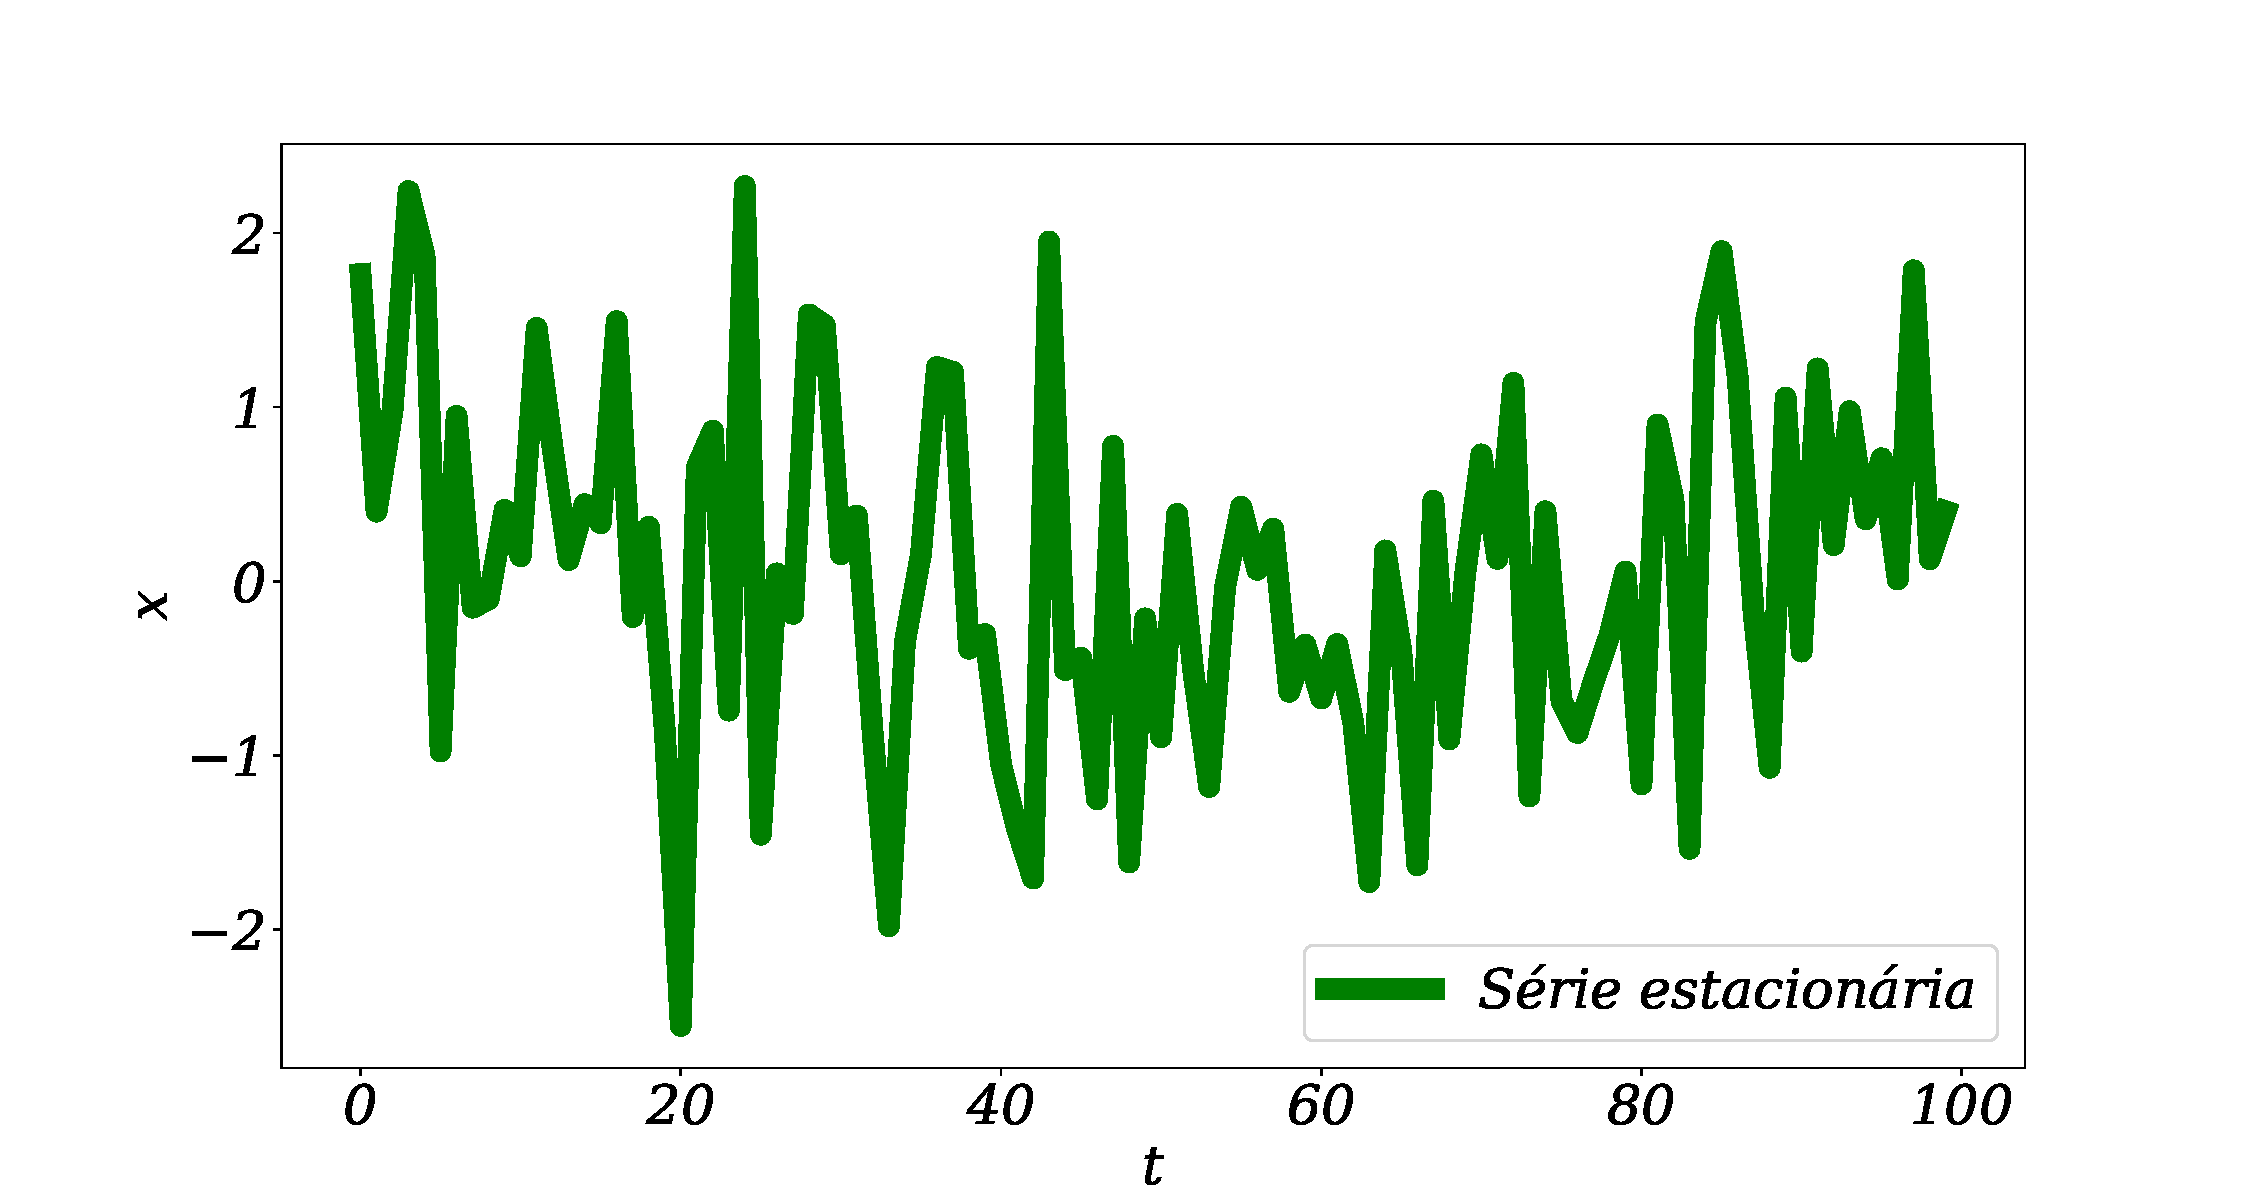
\includegraphics[width=\linewidth]{Revisao/Figuras/serie_estacionaria}
		\caption{Série estacionária com média}
	\end{subfigure}	\hfill
	\begin{subfigure}{0.39\textwidth}
		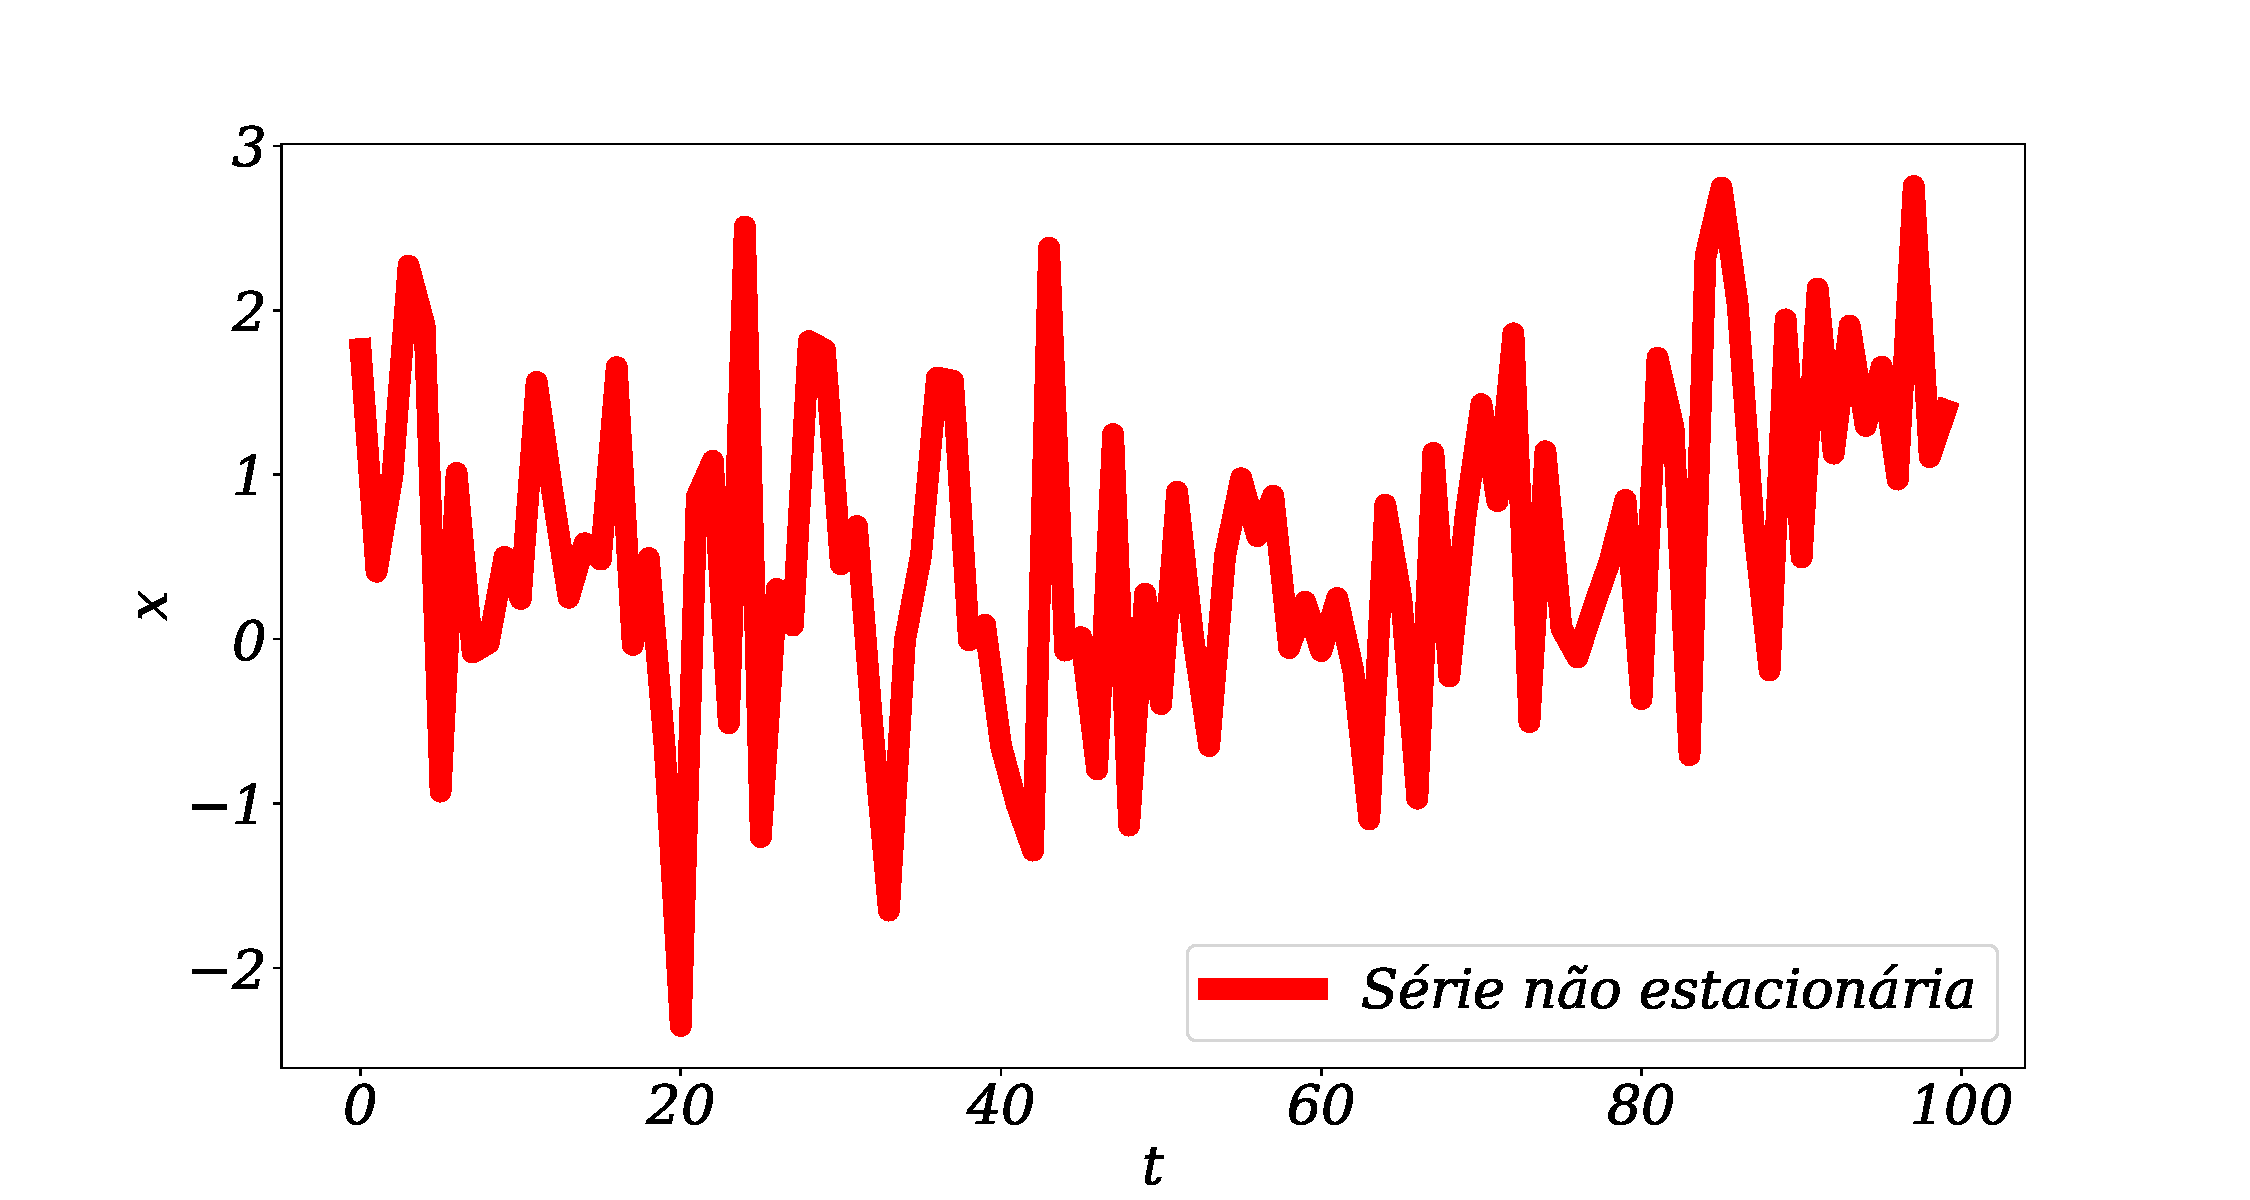
\includegraphics[width=\linewidth]{Revisao/Figuras/serie_nao_estacionaria_1}
		\caption{Média dependendo do tempo zero}
	\end{subfigure}
	
	\begin{subfigure}{0.39\textwidth}
		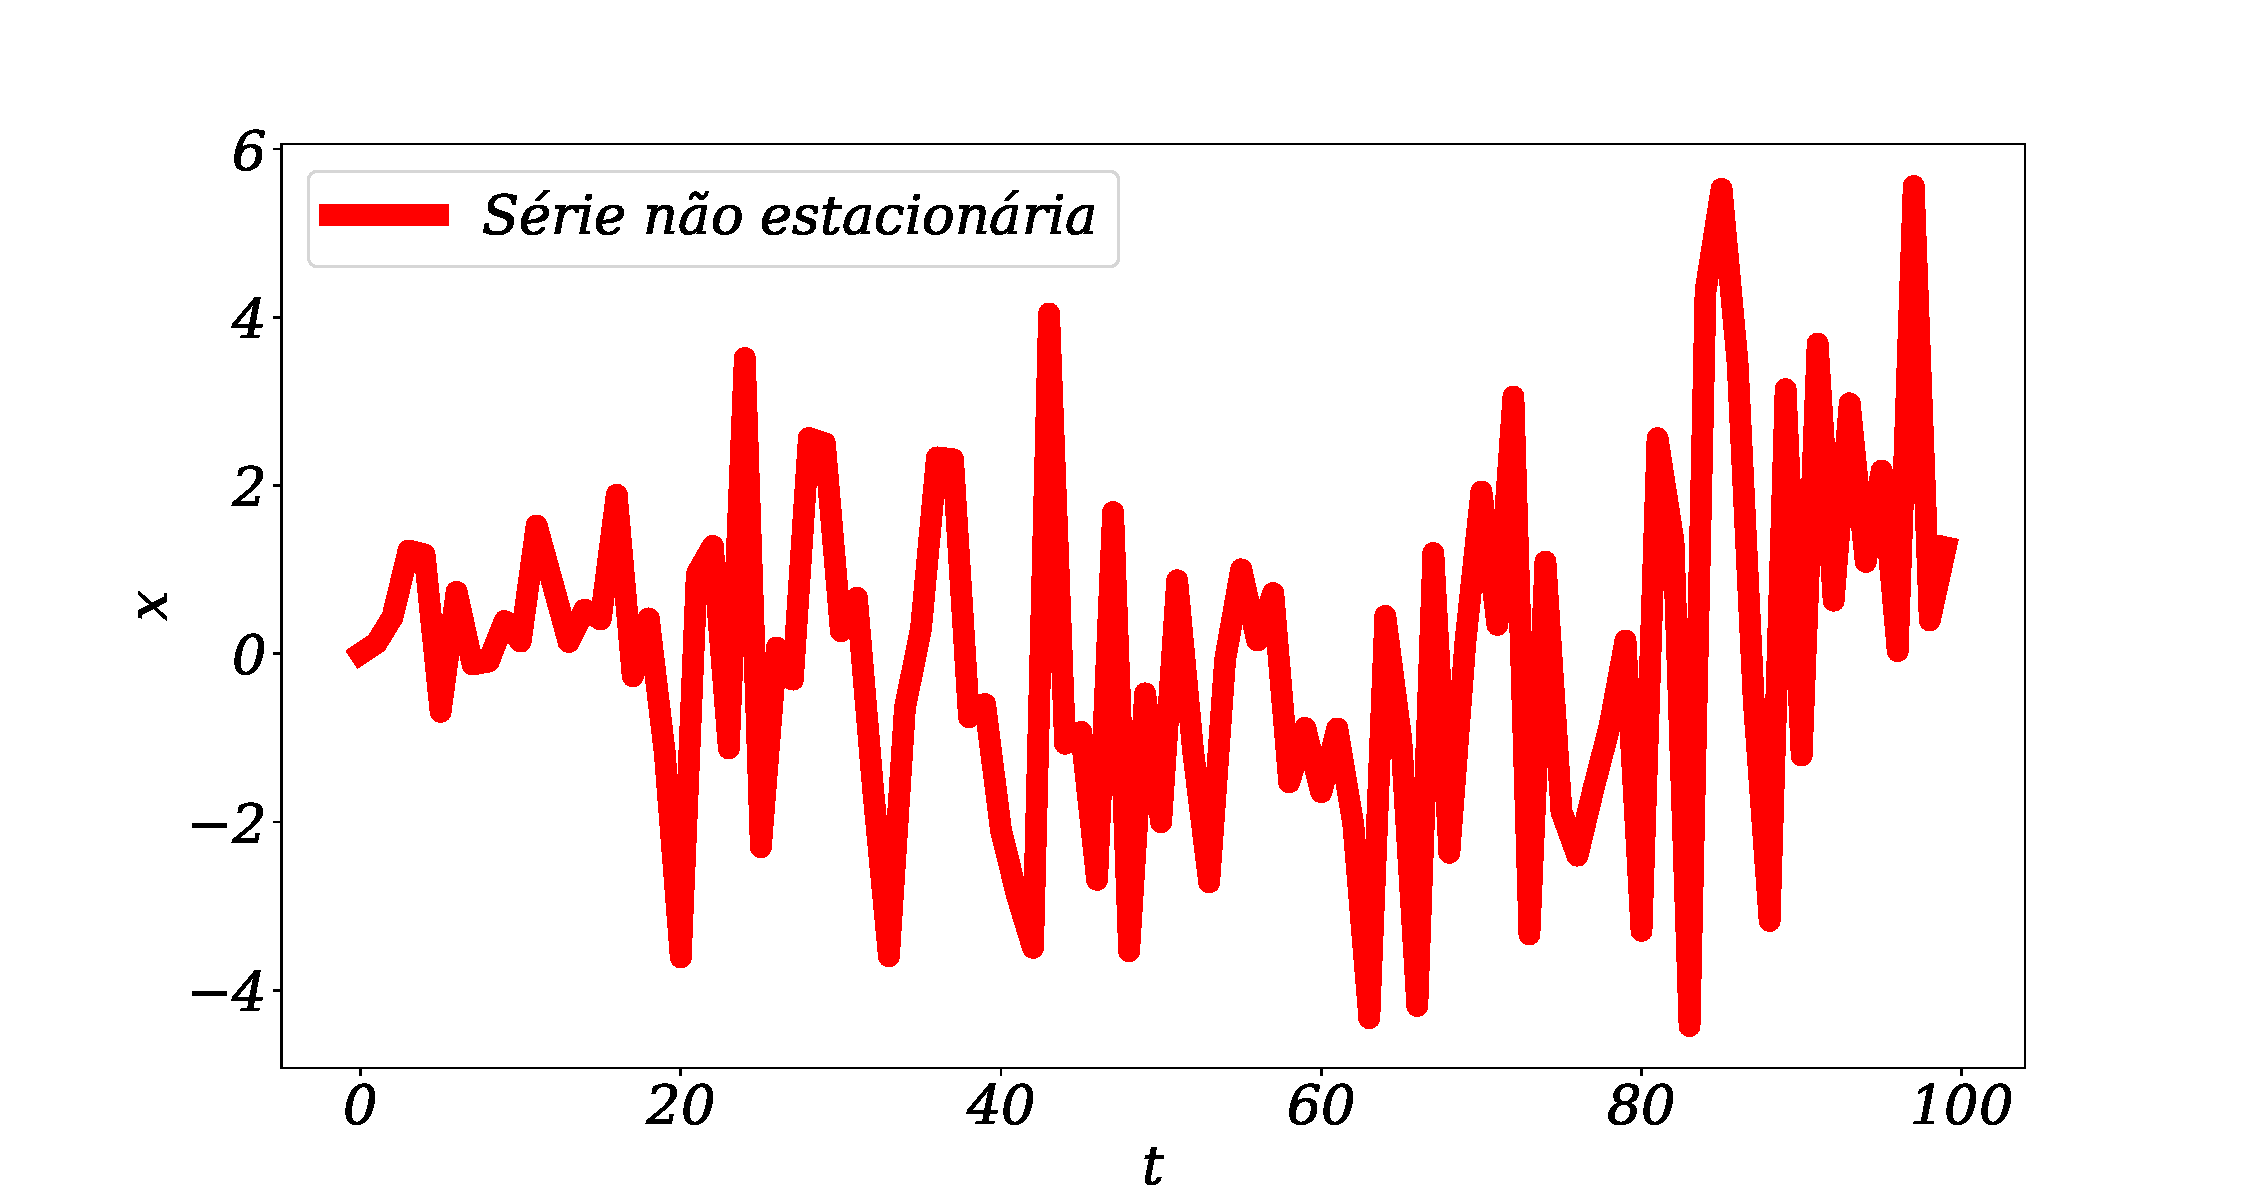
\includegraphics[width=\linewidth]{Revisao/Figuras/serie_nao_estacionaria_2}
		\caption{Variância dependendo do tempo}
	\end{subfigure}	\hfill
	\begin{subfigure}{0.39\textwidth}
		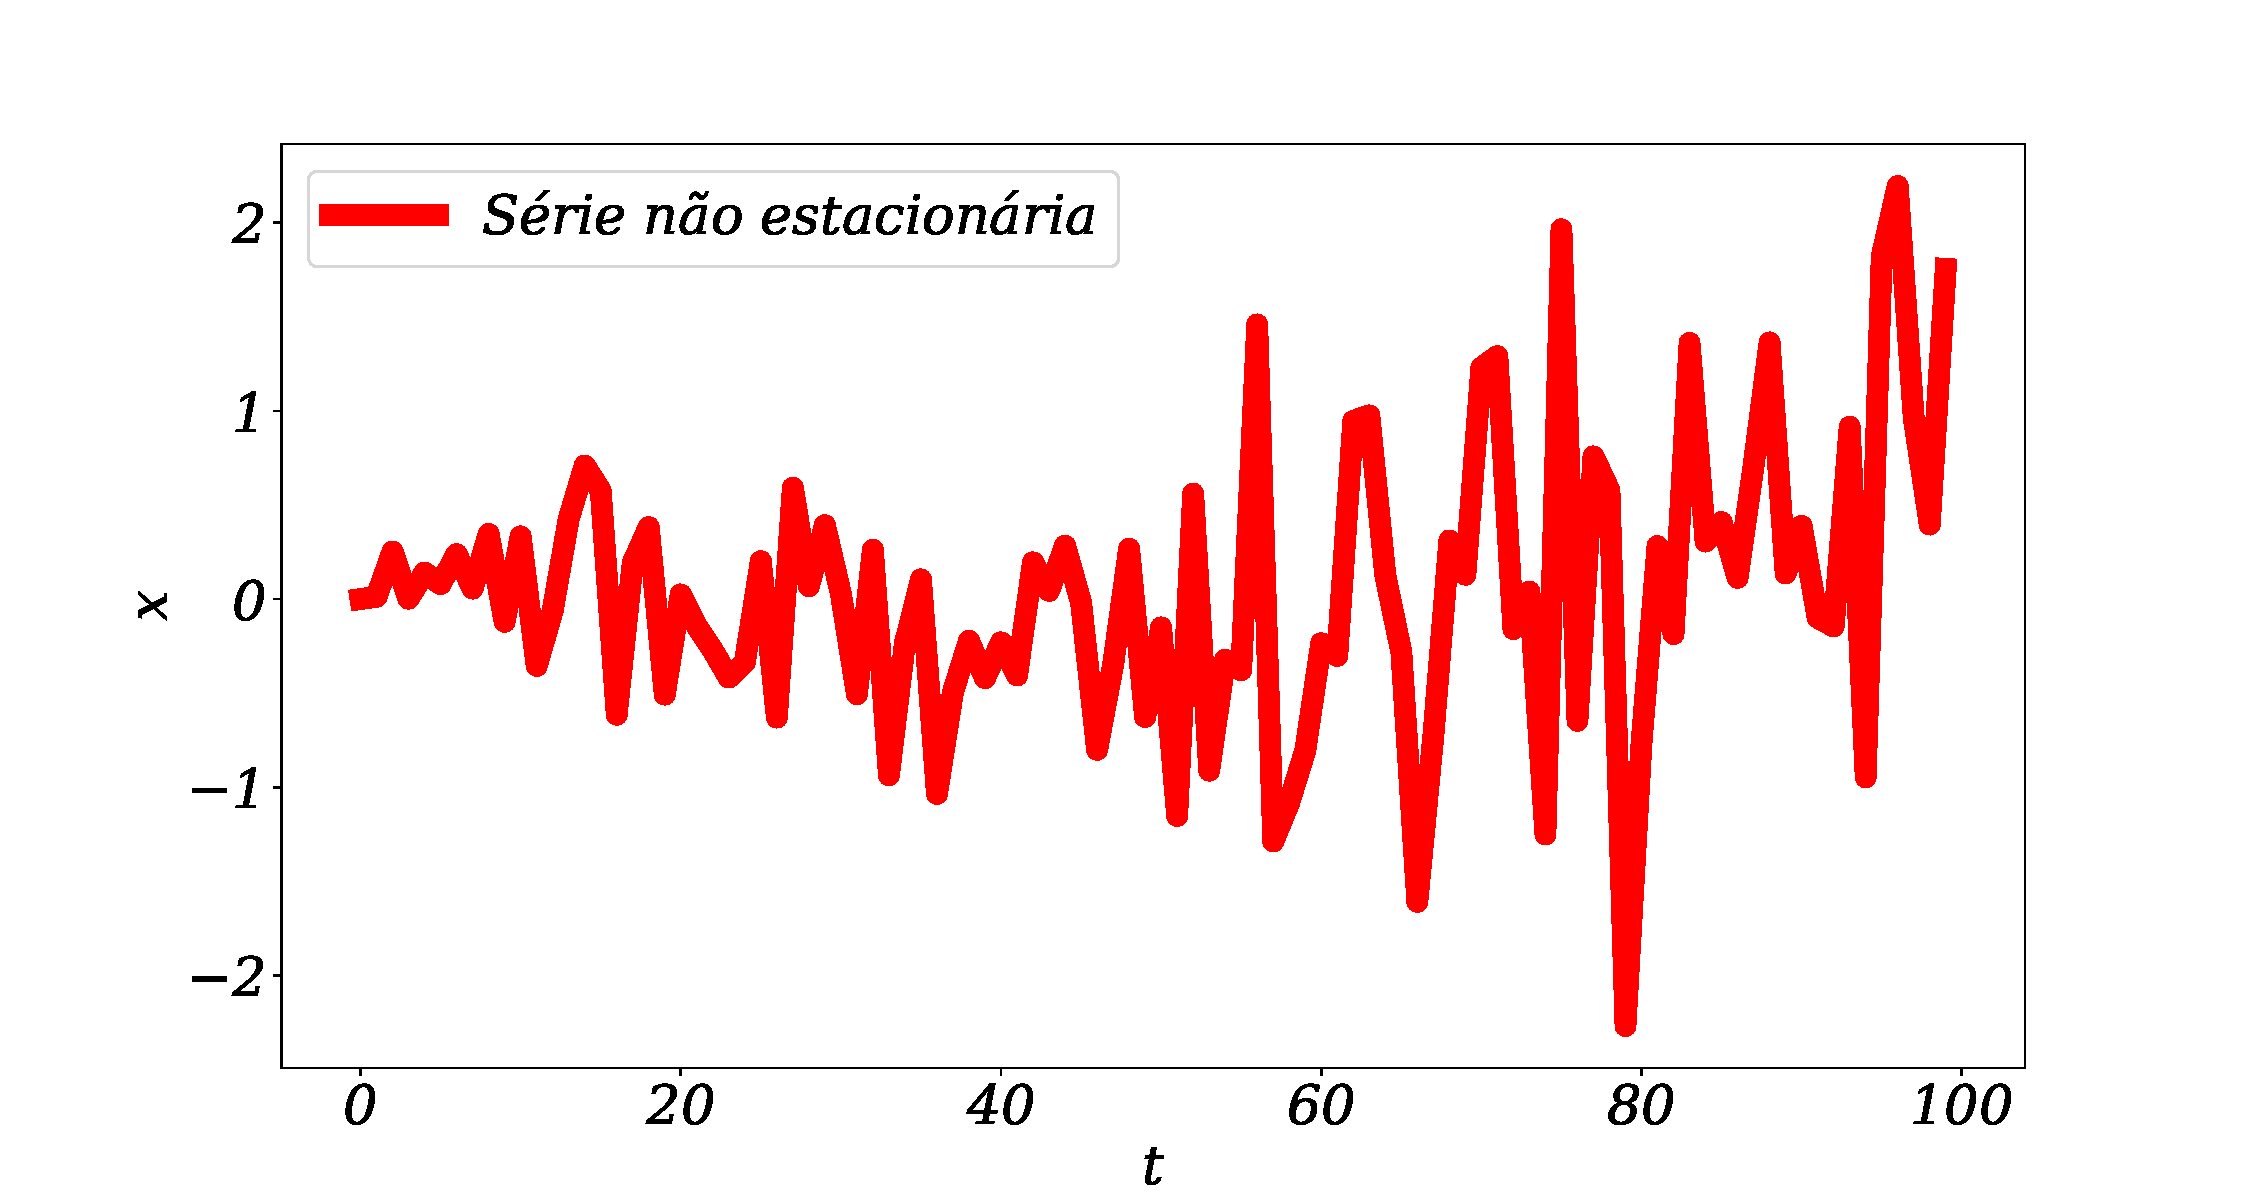
\includegraphics[width=\linewidth]{Revisao/Figuras/serie_nao_estacionaria_3}
		\caption{Covariância dependendo do tempo}
	\end{subfigure}
	

\fonte{Adaptado de \citeonline{brandão_2020}}
\end{figure}

	
		
